\documentclass[tikz,border=3mm]{standalone}
\usepackage{pgfplots}
\pgfplotsset{compat=1.17}
\usepgfplotslibrary{groupplots}
\usetikzlibrary{arrows.meta,positioning,fit,shapes.geometric,calc,backgrounds}
\begin{document}

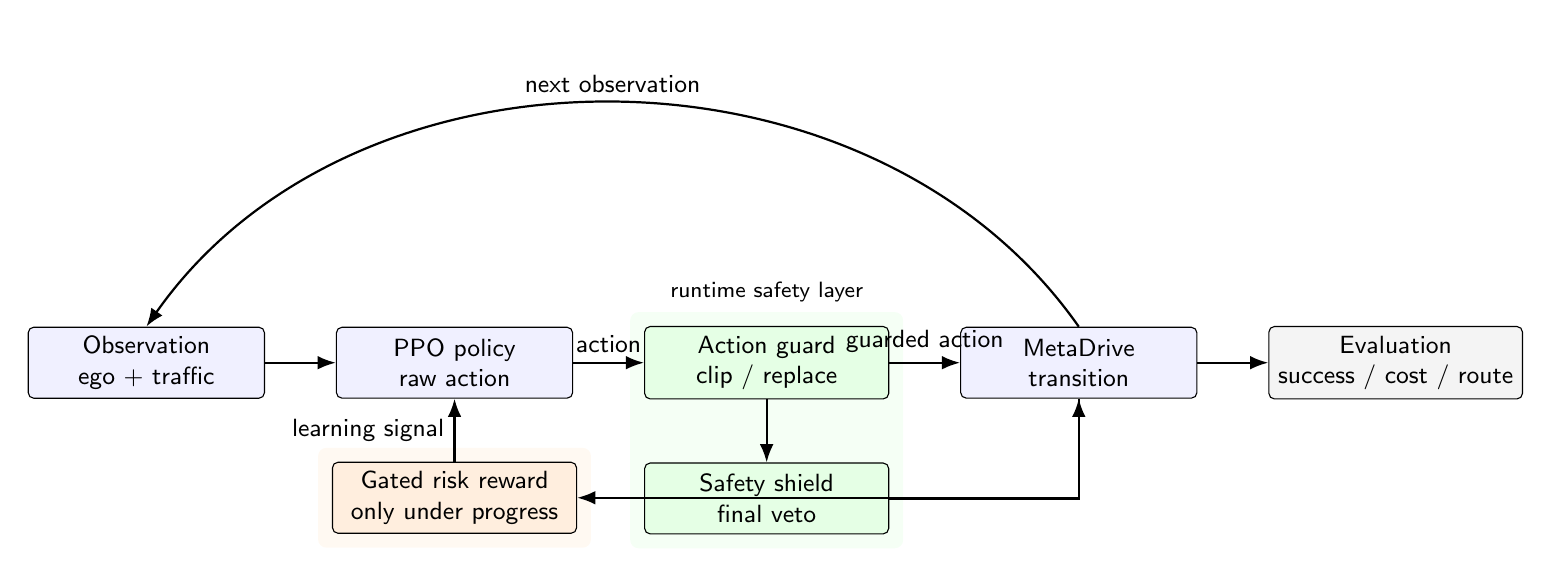
\begin{tikzpicture}[font=\sffamily\small, >=Latex,
module/.style={draw, rounded corners=2pt, fill=blue!6, minimum width=30mm, minimum height=9mm, align=center},
safe/.style={draw, rounded corners=2pt, fill=green!10, minimum width=31mm, minimum height=9mm, align=center},
risk/.style={draw, rounded corners=2pt, fill=orange!13, minimum width=31mm, minimum height=9mm, align=center},
metric/.style={draw, rounded corners=2pt, fill=gray!9, minimum width=30mm, minimum height=9mm, align=center}]
\node[module] (obs) {Observation\\ego + traffic};
\node[module, right=9mm of obs] (ppo) {PPO policy\\raw action};
\node[safe, right=9mm of ppo] (guard) {Action guard\\clip / replace};
\node[safe, below=8mm of guard] (shield) {Safety shield\\final veto};
\node[module, right=9mm of guard] (env) {MetaDrive\\transition};
\node[risk, below=8mm of ppo] (reward) {Gated risk reward\\only under progress};
\node[metric, right=9mm of env] (eval) {Evaluation\\success / cost / route};
\begin{scope}[on background layer]
\node[fill=green!4, rounded corners=3pt, fit=(guard)(shield), inner sep=5pt, label={[font=\sffamily\footnotesize]above:runtime safety layer}] {};
\node[fill=orange!5, rounded corners=3pt, fit=(reward), inner sep=5pt] {};
\end{scope}
\draw[->, thick] (obs) -- (ppo);
\draw[->, thick] (ppo) -- node[above]{action} (guard);
\draw[->, thick] (guard) -- node[above]{guarded action} (env);
\draw[->, thick] (guard) -- (shield);
\draw[->, thick] (shield.east) -| (env.south);
\draw[->, thick] (env) -- (eval);
\draw[->, thick] (env.south) |- (reward.east);
\draw[->, thick] (reward) -- node[left]{learning signal} (ppo);
\draw[->, thick, rounded corners=10pt] (env.north) to[out=125,in=55] node[above]{next observation} (obs.north);
\end{tikzpicture}

\end{document}
